\chapter{Related Work}

In this chapter, we will present several tools with similar focus as our proposed \emph{application generator}. That will help us to identify the key features that we will need to implement in order to achieve our goals. We aim to create a \emph{Linked Data-driven web application generator}. So we have to begin with defining what kind of tools would fall into the same category. Before we start: Let us not limit ourselves only to Linked Data based tools. Firstly, there is not that many similar Linked Data based tools available so there would not be much to analyze. Secondly, we can get interesting findings even from the other tools, as the inner data format is only one aspect of a generator (and for a non-developer, i. e., our potential user, it is definitely not the most important one). We will now move on to the individual features that a tool should have in order to be classified by us as a \emph{data-driven application generator}.

Firstly, such a tool should be a \emph{generator}. That means that whatever the generator produces, it should not disappear after the generator is closed and it should persist as an independent \emph{instance}. This requirement is rather vague as for example any text processor t(e.g. Microsoft Word) would count as a generator in this sense. But it does rule out all kinds of \emph{data viewers}. Secondly, such a tool should generate \emph{applications}. An application, to be called an \emph{application}, should offer (at least potentially) some level of interactivity. For example text documents, images or static visualizations (like non-interactive graphs) are definitely not applications. Lastly, such a tool should be \emph{data-driven}. That means that in a typical scenario, one should start the process with a data set and use this data set to create a new application with the generator.  To give you an example of what we do not consider \emph{data-driven}, we could mention for example the WordPress.com \cite{wordpress} platform. This platform definitely is an \emph{application generator} according to our first two requirements (specifically, it is a \emph{website generator}, or perhaps a \emph{blog generator}). The key difference is that when you create a new application (\emph{website} or \emph{blog}), it is completely empty and then you start adding the data. The process is completely reversed.

We admit that all these definitions are rather vague and it can still be hard to determine whether a certain tool falls into the category of \emph{data-driven application generators}. We believe, however, that all these definitions together give the reader a decent idea of what we consider a \emph{data-driven application generator}.

To make the comparison more organized, we define a limited set of features that we will specifically focus on while examining the tools. An overview table showing the support of these features among all selected tools will be presented to the reader at the end of this chapter. Let us now give a short description of each chosen feature.

\begin{itemize}
\item \emph{Linked Data support}. Our \emph{application generator} is going to be Linked Data based and we consider this aspect one of its biggest assets. Therefore we are naturally interested in the \emph{Linked Data support} of other tools as well.
\item \emph{Extendability}. We want to know whether a particular tool can be programmatically extended to support new types of data and new corresponding types of applications. By a type of data we do not mean a different format (the data might or might not be represented in RDF, that is irrelevant at this moment) but a different \emph{semantic} meaning of the data. For example, if we decide that our generator should be able to recognize geospatial data and visualize them using an application in the form of a map, can we extend the generator in such a way? Also just because a particular tool is released under an Open-source software license and therefore can be modified, we do not consider it \emph{extendable}. Such a tool has to be intentionally \emph{designed} as \emph{extendable} with clearly defined and document plugin interface.
\item \emph{Online sharing}. We want to know whether a generated application can be published online.
\item \emph{Non-developers friendly}. Here we are interested in whether the \emph{application generator} can be operated by a person with no technical knowledge. We are focused specifically on the actual application creation process. An expert might be needed to set up the generator, but this requirement would not break our condition.
\item \emph{Platform}. This feature specifies whether the generator exists in the form of an online \emph{platform} where each user has an account through which he can create, publish and manage his applications.
\item \emph{Configuration}. Here we want to know whether the generator will simply take the input data and generate and publish the application from it, or whether it will offer the user an extra \emph{configuration} step in between, in which the user will be able to affect the final shape of the application before publishing it. This configuration step should allow more than just changing the application name.
\end{itemize}

\def\checkmark{\tikz\fill[scale=0.4](0,.35) -- (.25,0) -- (1,.7) -- (.25,.15) -- cycle;}
\newcolumntype{C}{>{\centering}X} % Create new column type that centers the cell content
\begin{table}[ht]
  \caption{Features of related tools}
  \vspace{0.5cm}
  \label{tab:related-features}
\begin{tabularx}
  {\textwidth}{ |r|C|C|C|C|C|C| }
  \hline
      \begin{sideways}Tool\end{sideways} & 
      \begin{sideways}Linked Data support\end{sideways} &
      \begin{sideways}Extendability\end{sideways} &
      \begin{sideways}Online sharing\end{sideways} &
      \begin{sideways}Non-developers friendly\end{sideways} &
      \begin{sideways}Platform\end{sideways} &
      \begin{sideways}Configuration\end{sideways} \tabularnewline \hline
  \hline
% 						&LD			&Extend		&Sharing	&Non-devel	&Platform	&Config	
  Miga Data Viewer		&			& 			&\checkmark &			&			&\checkmark ~ \tabularnewline \hline
  Citadel on the Move	& 			&\checkmark	&\checkmark	&\checkmark	&\checkmark	&\checkmark	~ \tabularnewline \hline
  Tableau       		& Y~& Y~& A~& N~& Y~& W~ \tabularnewline \hline
  Avelca                & Y~& N~& - & N~& N~& W~ \tabularnewline \hline  
  Exhibit             	& N~& - & - & N~& - & W~ \tabularnewline \hline
  Payola              	& N~& - & - & N~& - & W~ \tabularnewline \hline
  LinkedPipes           & N~& - & - & N~& - & D~ \tabularnewline \hline

  
\end{tabularx}
\end{table}

\section{Miga Data Viewer}

Miga Data Viewer is a tabular data based \emph{application generator}. It accepts only data in the CSV format but as this format is widely supported and there is lots of conversion tools available, any source of tabular data (Microsoft Excel file, RDBMS) can be used as an input. Despite the word \emph{viewer} in the name, this tool does meet our requirements to be called an \emph{application generator}. What it generates is an interactive interface that supports browsing, searching and filtering over the input data set. Once it is generated, it can be published online.

\begin{figure}
	\centering
	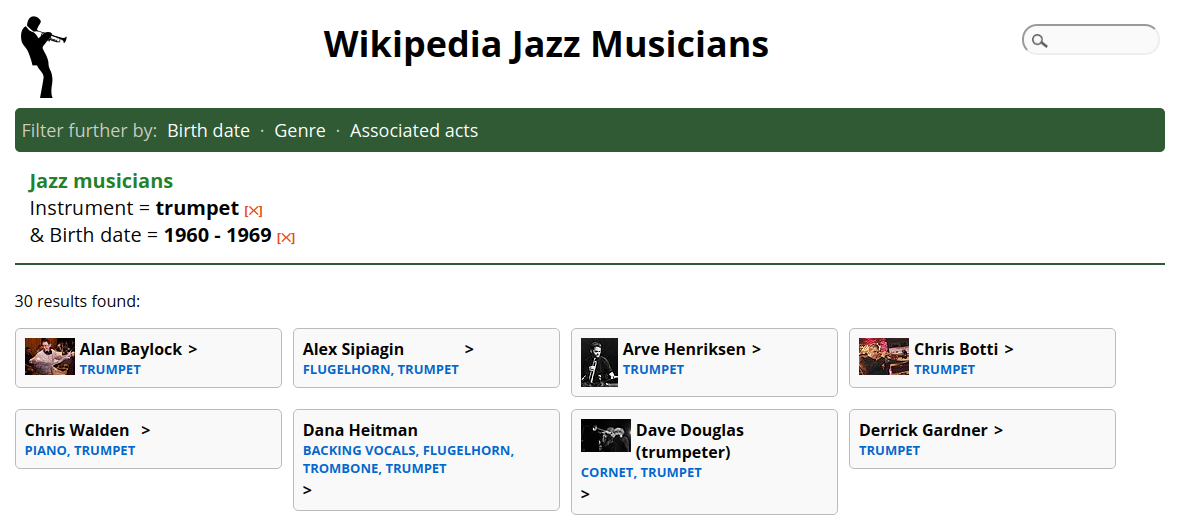
\includegraphics[width=140mm]{img/02_miga_data_viewer.png}
	\caption{Miga Data Viewer: A sample application generated from a set of Jazz Musicians.}
	\label{fig:miga-data-viewer}
\end{figure}

As we already mentioned in the introduction chapter, the big disadvantage of tabular data is that they carry very little semantic information. As without the semantic information, it would be almost impossible to generate anything else but a simple paginated table, the user is required to provide a \emph{schema definition} for each data table (for each single CSV file). That is done through configuration *.ini files using a custom \emph{Miga Data Schema} format. Here is an example of such a configuration:

\scriptsize
\begin{verbatim}
[Books]
Title = Name
Author = List (,) of Entity (Authors/Name)
Number of pages = Number
Genre = List (,) of Text
Wikipedia URL = URL

[Authors]
Name = Name
Birth date = Date
\end{verbatim}
\normalsize

Each section defines a scheme for a CSV file with a name matching the section's name. Each column in the data file is assigned one of the data types provided by the \emph{Miga Data Schema}. Besides the very basic ones (\emph{Text} or \emph{Number} that correspond to data types known from programming languages) and slightly more complex ones (\emph{List} for collections, \emph{Entity} working as a \emph{foreign key} pointing to a different CSV file), there are a few special ones with added \emph{semantic meaning}. Let us name for example \emph{URL}, \emph{Image URL} or \emph{Coordinates} (GPS coordinates). Using these types the Miga Data Viewer is able to create richer interfaces (e.g. it can display entities with coordinates on a map).

It is clear that this format is the authors' attempt to solve what RDF would be perfect for. But unlike RDF, which is a universal, open and widely supported framework, this format will work with Miga Data Viewer only. We will see similar approaches in other generators as well.

Although creating an application does not require the user to know any programming language, the process does involve fairly low-level work with the *.ini scheme files. Because of this we do not consider this tool \emph{non-developers friendly}.

\section{Citadel on the Move}

Citadel on the Move \cite{citadel_home} is a project \cite{citadel_paper} funded by European Commission. The presented goal is to simplify the process of generating Open Data based applications for both developers and non-developers, that provide useful city services. The idea behind this project was that an application providing a certain service (e.g. available park places) for one European city should be able to work just as well in another European city, only with a different data set. The applications generated by this tool are very simple map applications that work as interactive data viewers (similarly to Miga Data Viewer).
% * <tobiaspotocek@gmail.com> 2016-06-12T19:44:03.785Z:
%
% > Open Data
%
% How to reference this?
%
% ^.

\begin{figure}
	\centering
	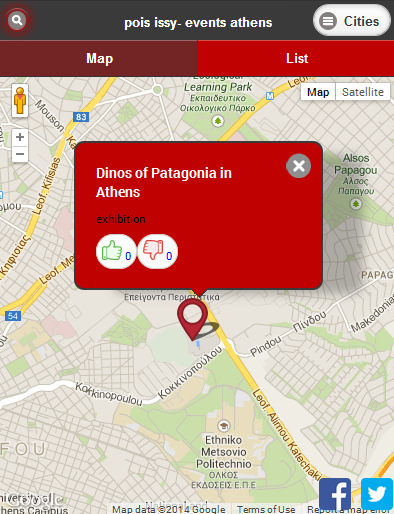
\includegraphics[width=80mm]{img/02_citadel_on_the_move_app.jpg}
	\caption{Citadel on the Move: A sample generated application. Source of picture \cite{citadel_agt_doc}}
	\label{fig:citadel-on-the-move}
\end{figure}

Citadel on the Move is not a monolithic application but a fairly large project consisting of several components.

\begin{itemize}
\item The project defines its own data set format called \emph{Citadel JSON}. As the name suggests, the data are serialized into JSON following a custom scheme. Each data set contains a single list of entities where each entity has couple of mandatory fields (like an ID, name or GPS coordinates necessary for the map visualization) plus an arbitrary number of optional attributes (which may vary depending on a data set and are not in any way defined by the scheme). 
\item The project offers a \emph{Citadel table to JSON Converter tool} which allows the user to convert any tabular data (typically CSV or XLS) into the internal {Citadel JSON} format. Clearly, the original data set has to contain all required information. The tool just enables the user to create mappings between table columns of the original data set and the schema fields.
\item The core component is the \emph{Application Generator Tool} which allows non-developers to create their own application in just couple of simple steps. They start by selecting a city (or cities) that they are interested in, they continue by selecting a data set (or data sets) available for the chosen city (or cities) and finally they just fill in basic app configuration (name, description, color scheme) to create the application. The generated application is an interactive interface that allows the user to browse, filter and see the data on a map (as said, similarly to Miga Data Viewer).
\item A part of the project is also a \emph{platform} in a form of an online portal available on the cited URL \cite{citadel_home}. It is wrapped around the  \emph{Application Generator Tool} and provides additional functionality like published applications catalog, user management, support etc.
\item The last component are customizable application \emph{templates}. If the application generated by the \emph{Application Generator Tool} is not sufficient, the user can instead manually instantiate a \emph{template} and configure it to use the given data set. This approach is completely separated from the \emph{Application Generator Tool}. It is not possible to select a template while generating an application. This has to be done manually and it requires certain programming skills. A distinct advantage is that using a template gives the user significantly bigger freedom of customization. E.g. it is possible to edit the application's layout or upload a custom application logo. An example of such a special template is the \emph{Citadel Events Template} that extends the default application (which is used in the \emph{Application Generator Tool}) by a calendar which allows filtering over events contained in the data set (those are standard entities with couple extra attributes that are specified in the template documentation).
\end{itemize}

To sum it up: Citadel on the Move offers two different approaches. The first one utilizes the \emph{Application Generator Tool} which allows non-developers to generate simple applications in a very \emph{friendly} way. The other one utilizes the \emph{templates} which allow developers to create more customizable applications. There is no data \emph{analysis} involved. The user has to select a different template manually and he has to make sure that the given data set contains all necessary information that the template needs in order to work properly. The project offers several different documented templates and encourages the developers to create new ones which makes the project \emph{extensible}. As the \emph{templates} are just standalone web applications (not plugins), there is no interface that they would need to implement. However, they need to support the common \emph{Citadel JSON} format. Just like Miga Data Viewer, Citadel on the Move needs to address the problem that standalone tabular data contain almost no semantic information. To deal with that, it provides the \emph{JSON Converter tool} which allows the user to map the data set table columns onto the Citadel JSON scheme.



